%% Copyright 2019 Matheus H. J. Saldanha <mhjsaldanha@gmail.com>
%
% This work may be distributed and/or modified under the
% conditions of the LaTeX Project Public License, either version 1.3
% of this license or (at your option) any later version.
% The latest version of this license is in
%   http://www.latex-project.org/lppl.txt
% and version 1.3 or later is part of all distributions of LaTeX
% version 2005/12/01 or later.
%
% This work has the LPPL maintenance status `maintained'.

\documentclass[12pt,a4paper]{article}

% Pacotes para o português.
\usepackage{rotating}
\usepackage[brazilian]{babel}
\usepackage[utf8]{inputenc}
\usepackage[T1]{fontenc}
\usepackage{float}
\usepackage{graphicx}     % Comando \includegraphics
\usepackage{xcolor}       % Comando de cores \textcolor
\usepackage{indentfirst}  % Indenta o primeiro parágrafo de cada seção
\usepackage{url}          % Comandos \url e \href
\usepackage[top=2cm, bottom=2cm, left=2cm, right=2cm]{geometry} % Define as margens do documento
\usepackage{multirow}     % Permite criar tabelas com uma célula ocupando várias linhas
\usepackage{amssymb}      % Símbolos matemáticos
\usepackage{amsmath}      % Ambientes para escrever fórmulas, \begin{align} por exemplo.
\usepackage{caption}      % Para definir o estilo das legendas de figuras e tabelas.
\usepackage{setspace}     % Para definir espaçamento entre linhas. (\onehalfspacing, \singlespacing, \doublespacing)
\usepackage{breakcites}   % Para permitir quebra de linha no meio de citações.
\usepackage{times}        % Fonte Times New Roman
\usepackage{lipsum}       % Para gerar texto temporário. Exemplo: \lipsum \lipsum[1] \lipsum[4-5].
\usepackage{inconsolata}  % Fonte boa para códigos e URLs. Use \texttt{}
\usepackage{hyperref}     % Faz os links ficarem azuis e clicáveis. Facilita a navegação pelo PDF.

\makeatletter
\hypersetup{
	pdfkeywords={research project},
	colorlinks=true,       		% false: boxed links; true: colored links
	linkcolor=blue,          	% color of internal links
	citecolor=blue,        		% color of links to bibliography
	filecolor=magenta,      	% color of file links
	urlcolor=blue,
	bookmarksdepth=4,
}
\makeatother

\makeatletter
\renewcommand\tableofcontents{%         % Redefine table of contents to our taste
    \section*{\huge\centering\contentsname
        \@mkboth{%
           \MakeUppercase\contentsname}{\MakeUppercase\contentsname}}%
           \vspace{24pt}%
    \@starttoc{toc}%
    \newpage%
}

% Comando para marcar o texto para revisão.
\newcommand{\rev}[1]{\textcolor{red}{#1}}

% Permite escrever aspas normais "text" em vez de ``text''
\usepackage[autostyle]{csquotes}
\MakeOuterQuote{"}

\begin{document}

\doublespacing

\begin{titlepage}
\begin{figure}[H]
    \centering
    
\includegraphics[scale=0.4]{imagens/cemaden.png}
    \label{fl}
\end{figure}
    \begin{center}
        {\large \sc CENTRO NACIONAL DE MONITORAMENTO E ALERTAS \\ DE DESASTRES NATURAIS - CEMADEN} \\
        {\large \sc }\\[0.7cm]
        {\small \sc }
        
        \vspace{4cm}

        % Título.
        {\large \sc Projeto de Pesquisa FAPESP}\\
        \rule{\linewidth}{2pt}
        
        \vspace{0.7em} % Ajuste ao seu gosto
        {\Large \bfseries APLICAÇÃO DE APRENDIZADO DE MÁQUINA PARA PREVISÃO DE ALAGAMENTOS}
        \vspace{0.2em} % Ajuste ao seu gosto
        
        \rule{\linewidth}{2pt} \\
        {\small \sc Linha de Fomento: Bolsa no País - Regular - Iniciação Científica}
    \end{center}

    \vspace{2.8cm}

    % Assinaturas
    \begin{minipage}{0.43\textwidth}
        \emph{Candidato:}\\[2.08cm]
        \rule{0.9\linewidth}{0.3mm}\\
        Vitor Yuichi Hossaki
    \end{minipage}
    \hspace{1cm}
    \begin{minipage}{0.43\textwidth}
        \emph{Orientador:}\\[2.08cm]
        \rule{0.9\linewidth}{0.3mm}\\
        Prof. Dr. Leonardo Bacelar Lima Santos
    \end{minipage}

    \vfill

    % Data
    \begin{center}
        \makeatletter
        São José dos Campos, SP \\
        \@date
        \makeatother
    \end{center}

\end{titlepage}
\tableofcontents
\newpage
\setcounter{page}{1}
\pagestyle{plain} % Agora passa a numerar as páginas

\section{Introdução}
\label{section:introducao}
%%%%%%%%%%%%%%%%%%%%%%%%%%%%%%%%%%%
\chapter{Introdu��o}
Os alagamentos s�o fen�menos cada vez mais frequentes em regi�es urbanas devido ao aumento da popula��o e o crescimento desordenado do processo de urbaniza��o. Em S�o Paulo, os alagamentos s�o recorrentes desde os prim�rdios de sua ocupa��o, a estrutura urbana aliado �s caracter�sticas dos rios existentes auxiliam na deflagra��o destes fen�menos \cite{hirata2013mapeamento}. Segundo \cite{santos2013impactos}, estima-se que os efeitos macroecon�micos dos alagamentos s�o de 172.3 milh�es de reais por ano, afetando setores log�sticos e industriais.

Diante dos impactos materiais, econ�micos e humanos causados pelos alagamentos, � necess�rio medidas que visem a mitiga��o e antecipa��o deste fen�meno. Estas medidas est�o associadas a uma infinidade de maneiras como os sistemas de alertas, essencial para que a comunidade seja alertada com anteced�ncia de fen�menos naturais intensos e, desta forma, minimizar e previnir poss�veis danos materiais e humanos \cite{kobiyama2006prevenccao}. 

Nesse �nterim, algumas pesquisas como de \cite{horita2015development} e  \cite{hirata2013mapeamento}, demonstram que a utiliza��o de redes sociais que cont�m informa��es geogr�ficas volunt�rias, podem ser um instrumento efetivo para o desenvolvimento de sistemas monitoramento e alertas das poss�veis ocorr�ncias de alagamento.

O autor \cite{de2015geographic} demonstra a potencialidade da rede social Twitter para a gest�o de desastres, combinando-se dados hist�rico espa�o temporais desta rede. As postagens s�o filtradas atrav�s de palavras chaves e classificadas binariamente como relacionado ou n�o-relacionada, aliando-se � s�rie temporal de deflagra��es dos alagamentos em determinada regi�o. Neste contexto, os dados s�o analisados estatisticamente atrav�s de GLMs (modelos lineares generalizados). Por fim, o trabalho indica a relev�ncia estat�sticas dos Tweets relacionados, pr�ximos �s regi�es de alagamento ($\leq10km$ do local de ocorr�ncia). 

Al�m disso, � verificado uma ascens�o na literatura quanto ao emprego de intelig�ncia artificial, principalmente o Machine Learning, para a gest�o e tomada de decis�o em desastres. Na pesquisa de \cite{sit2019identifying}, s�o utilizados algoritmos de processamento de linguagem natural para identificar a sem�ntica de Tweets relacionados ao contexto de desastres. O aprendizado de m�quina tamb�m � incorporado para analisar m�ltiplos par�metros f�sicos para a previs�o de alagamentos \cite{mosavi2018flood}.

Em face do crescimento da utiliza��o de intelig�ncia artificial e das consequ�ncias dos alagamentos, a finalidade deste projeto � definir qual � o algoritmo de aprendizado de m�quina que possui maior precis�o com rela��o � previs�o de alagamentos, utilizando-se um conjunto de atributos aliado � rede social Twitter. 

A estrutura geral da proposta � dividida e enunciada a seguir; na Se��o 2 � esclarecido qual � o objetivo principal e espec�fico do trabalho; na Se��o 3 a relev�ncia e import�ncia do tema proposto;  sobre as quest�es centrais abordadas no trabalho e conceitos explicado de maneira mais espec�fica s�o encontradas na Se��o 4; a Se��o 5 � de destinada � delimita��o da �rea de estudo e a disponibilidade e origem dos dados e a metodologia prevista;  por fim na se��o 6 � encontrada o plano de atividade e cronograma. 



\section{Objetivos}
\label{section:problemapsp}
%%%%%%%%%%%%%%%%%%%%%%%%%%%%%%%%%%%
\chapter{Objetivos}

A finalidade deste projeto � alinhar-se com os objetivos do Centro Nacional de Alerta de Desastres Naturais (CEMADEN) no desenvolvimento de meios para prever alagamentos, partindo-se da hip�tese que � poss�vel utilizar algoritmos de aprendizado de m�quina para detectar alagamentos, e desta forma, emitindo-se alertas.


Objetivos espec�ficos: 
\begin{enumerate}
    \item Definir qual � o algoritmo mais preciso para relacionar os dados metereol�gicos, pluviom�tricos e frequ�ncia de tweets para o modelo de classifica��o de dias de alagamentos e n�o-alagamentos. 
\end{enumerate}




\section{Justificativa e relevância do projeto}
\label{section:hpc}
%%%%%%%%%%%%%%%%%%%%%%%%%%%%%%%%%%%
\chapter{Justificativa e Relev�ncia}

O  desenvolvimento  acelerado  de  S�o  Paulo  culminou  na  urbaniza��o  descontrolada causando diversas consequ�ncias na regi�o.   A impermeabiliza��o do solo,  a drenagem urbana deficit�ria e a topografia favor�vel ao ac�mulo de �gua,  s�o reflexos desta expans�o desordenada. A deflagra��o de alagamentos causaram diversas perdas diretas e indiretas para o PIB de S�o Paulo, alcan�ando m�dia de 172 milh�es de reais em preju�zos econ�micos por ano em algumas regi�es do estado. Diante dos danos humanos, materiais e econ�micos que os alagamentos v�m causando ao longo das d�cadas, � necess�rio medidas mitigadoras e o desenvolvimento de sistemas de alertas que possam antecipar a poss�vel deflagra��o do fen�meno hidrol�gico. 


Al�m disso, em virtude da ascens�o mete�rica da tecnologia e da influ�ncia das redes sociais, o projeto visa o desenvolvimento da computa��o aplicada aos fen�menos hidrol�gicos de alagamentos, utilizando-se conceitos de ci�ncia de dados e \textit{Machine Learning}.




\section{Fundamentação Teórica}
\label{section:trabrelacionados}
%%%%%%%%%%%%%%%%%%%%%%%%%%%%%%%%%%%
\chapter{Fundamenta��o Te�rica}

%%%%%%%%%%%%%%%%%%
\section{Alagamentos}
Os alagamentos s�o fen�menos associados ao ac�mulo de �gua em determinado local, favorecidos pela microdrenagem e macrodrenagem insuficientes. A aus�ncia de planejamento urbano e a r�pida modifica��o do espa�o culmina na impermeabiliza��o do solo, contribuindo para diminui��o do tempo concentra��o e o aumento do volume de escoamento superficial, amplificando-se assim, o pico da vaz�o e consequentemente saturando a drenagem pluvial do local \cite{hansmann2013descriccao}. 

A topografia e a eleva��o do local tamb�m s�o fatores preponderantes para a ocorr�ncia de alagamentos, ou seja, verifica-se que os lugares com maior frequ�ncia de alagamentos tem caracter�sticas morfom�tricas planas, depress�es ou fundos de vales, dificultanto o processo de escoamento superficial do local \cite{braga2016alagamentos}.

Fatores como o descarte inadequado de res�duos s�lidos, podem causar obstru��o dos sistema de drenagem do local, isto ocorre em decorr�ncia da aus�ncia de educa��o ambiental da popula��o. 

Os alagamentos s�o fen�menos complexos, uma vez que a sua causa est�  interrelacionada a uma gama par�metros como o clima que incluem precipita��o forte ou persistente, falhas estruturais urbanas, sistemas de drenagem inadequados, bacias hidrogr�ficas, proximidades de corpos aqu�ticos, uso e ocupa��o inapropriado do solo e entre outros \cite{doocy2013human}. 


%%%%%%%%%%%%%%%%%%
\section{A utiliza��o de redes sociais para o monitoramento de eventos}
O desenvolvimento da sociedade na esfera tecnol�gica permitiu a ascens�o mete�rica das redes sociais e suas funcionalidades. A quantidade massiva de dados gerados das redes sociais consolidam a intera��o do universo virtual com o mundo concreto, onde usu�rios expressam suas percep��es e emo��es acerca dos eventos circundantes \cite{naaman2011geographic}. A atividade das redes sociais e sua heterogeneidade espacial demonstra a potencialidade para o monitoramento de eventos metereol�gicos como a precipita��o \cite{de2021effect}. 

Atrav�s das plataformas de m�dia social, uma �nica postagem pode ser vista por milhares de usu�rios simultaneamente, al�m disso algumas plataformas utilizam-se de georreferenciamento que permite a visualiza��o n�o s� da postagem como tamb�m a localiza��o do usu�rio com seu dispositivo m�vel. Redes sociais (Twitter) ou aplicativos como Open Street Map que permitem a tecnologia de georreferenciamento s�o denominadas informa��es geogr�ficas volunt�rias, o trabalho de \cite{horita2015development}, integra estas plataformas para o gerenciamento de risco dos alagamentos. 

A utiliza��o das redes sociais apresentam uma crescente tend�ncia na sua incorpora��o em pesquisas para o monitoramento e an�lise de uma infinidade de eventos. Segundo \cite{de2015geographic}, a utiliza��o de informa��es geogr�ficas volunt�rias, principalmente a rede a social Twitter, s�o componentes fundamentais para a maior consci�ncia dos eventos ocorrentes ou seja, consolida-se a percep��o dos elementos no ambiente e possibilita maior compreens�o das poss�veis consequ�ncias. 
 
 
%%%%%%%%%%%%%%%%%%
\section{Classifica��o}
O Aprendizado de M�quina � cada vez mais empregado pelos pesquisadores na �rea de desastres de naturais, alguns autores utilizam esta ferramenta para analisar a sem�ntica atrelada das postagens de rede social, e assim, aprimorar os resultados da classifica��o de determinada ocorr�ncia \cite{de2015geographic, deparday2019machine}. 

Esta tecnologia pode ser definida como um conjunto m�todos computacionais para aprimorar performance ou realizar predi��es acuradas. A classifica��o � um dos m�todos computacionais amplamente utilizados para categoriza��o de cada item em uma s�rie de dados. Matematicamente, a classifica��o � descrita por uma fun��o \(F: \mathcal{X}\longrightarrow \mathcal{Y}\) que associa elementos no conjunto de atributos \(\mathcal{X}\) a uma classe de \(\Omega=\{\omega_1, \omega_2,...,\omega_n\}\), com \(n \in \mathbb{N}^*\), e partindo-se de um indicador de classe \(\mathcal{Y}=\{1,2,...,n\}\), portanto, quando \(x \in \mathcal{X}\) e \(y \in \mathcal{Y}\), a fun��o \(y=F(x)\) indica que x pertence � \(\Omega_y\).

Os modelos de aprendizagem supervisionada, a fun��o \(F\) utiliza-se das informa��es do conjunto de treinamento representado pela equa��o \(\mathcal{D}=\{(x_j,\omega_j \in \times \Omega : i=1,...m; \ j=1,...,c \}\), no qual \(m \) � a quantidade de dados no treinamento.


Atualmente os principais algoritmos empregados para classifica��o s�o o \textit{Suport Vector Machine} (SVMs) e \textit{Random Forest} \cite{mohri2018foundations}.

%-----------------
\subsection{Suport Vector Machines (SVMs)}
O m�todo SVM realiza a distin��o entre amostras de treinamento partindo-se de um hiperplano que possui maior abrang�ncia de separa��o, mapeando o padr�o de vetores para um espa�o de alta dimens�o, determinando-se o hiperplano mais adequado para separa��o de dados. Este algoritmo � utilizado por diversos autores devido � alta acur�cia para problemas de classifica��o bin�ria \cite{lian2006multi} . 

O hiperplano corresponde ao lugar geom�trico nos quais a fun��o \(f(x)=\langle w,x \rangle+b\) � nula. A vari�vel \(w\) � o vetor ortogonal ao hiperplano e \(b\) a dist�ncia entre a fun��o e a origem do espa�o de atributos. 

Para se encontrar o hiperplano mais adequado para separa��o entre as classes, � necess�rio a resolu��o do problema de otimiza��o \cite{theodoridis2010introduction} representado por:
\(
    max_\gamma (\sum^m_{i=1} \gamma_i-\frac{1}{2}\sum^m_{i=1}\sum^m_{j=1}\gamma_i \gamma_j y_i y_j \langle x_i,x_j \rangle), \ 
    \begin{cases}
0 \leq \gamma_i \leq \mathcal{C}, i=1,...,m \\
    \sum^m_{i=1} \gamma_i y_i=0
\end{cases}
\), 
a vari�vel \(\mathcal{C}\) � o par�metro utilizado para regulariza��o para ajustar o hiperplano e \(\gamma_i\) s�o os multiplicadores de Lagrange. 


A defini��o dos par�metros \(w\) e \(b\) que comp�em o hiperplano s�o dadas por: 
\(
    w=\sum_{\forall x_i \in SV}y_i \gamma_i x_i, \  
    b=\frac{1}{\#SV}(\sum_{x_i \in SV} y_i+ \sum_{x_i \in SV} \cdot \sum_{x_j \in SV} \gamma_i \gamma_j y_i y_j \langle x_i,x_j \rangle) 
\), \(SV\) � um subconjunto das amostrar de treinamento \(\mathcal{D}\), nos quais os elementos s�o os vetores suporte. Por fim indica��o da classe pertencente do vetor analisado � dado pelo sinal da fun��o discriminante \(f(x)\) \cite{maselli2019integraccao}.


%-----------------
\subsection{Floresta Aleat�ria (\textit{Random Forest})}
A classifica��o atrav�s do algoritmo Floresta Aleat�ria vem sendo amplamente utilizada literatura para avalia��o e mapeamento dos padr�es de eventos hidrol�gicos. Pesquisa como de \cite{zhu2021flood} e \cite{liu2020random} demonstram a potencialidade do algoritmo para avaliar a resili�ncia e os padr�es espaciais dos alagamentos. 


Este modelo � um algoritmo de classifica��o que representa um conjunto de �rvores de decis�o, que combina a sa�da destas diversas �rvores atribuindo-se uma classe ao conjunto de dados. Segundo \cite{breiman2001random}, a Floresta Aleat�ria consiste em uma cole��o de classificadores em forma de �rvore descritos por \(\{h(x,\theta_k), k=1,..\}\) onde \(\theta_k\) s�o independentes e em cada �rvore � lan�ado um voto unit�rio para a classe mais popular para o input \(x\). 


%-----------------
\subsection{Redes Neurais}
Este algoritmo vem sendo empregado para emiss�o de alertas hidrol�gicos e mapeamentos de suscetibilidade em alguns autores como \cite{da2016utilizaccao} e \cite{pacheco2020mapeamento}, demonstrando efetividade e acur�cia elevada para os modelo de previss�o associados aos fen�menos hidrol�gicos. 


A t�cnica \textit{Multilayer Perceptron} demonstra resultados relevantes as mais diversas �reas da ci�ncia \cite{gardner1998artificial}. Este algoritmo consiste em um sistema interconectado de neur�nios, estes n�s s�o conectados entre si por um peso. Matematicamente as camadas de neur�nios de entrada e sa�da s�o vetores definidos como $i$ e $O$ respectivamente, e os pesos como uma matriz $W$. Portanto a sa�da da rede � dada por $O=f(IW_{io})$, ao final do processo uma fun��o determina se aquele n� ser� ativado na condi��o $f(x)\begin{cases} 
1 \ \ x>0 \\
0 \ \ otherwise
\end{cases}$. Assumindo que $T$ � o par�metro de sa�da para o vetor de treinamento, o algoritmo o calcula o erro associado atrav�s de $E(O)=T-O=T-f(IW_{io})$. Algumas t�cnicas visam a redu��o do erro atrav�s da atualiza��o dos pesos no processo representado matematicamente por $W_{io}(t+1)=W_{io}(t)+\alpha E_n$.






\section{MATERIAIS E MÉTODOS}
\label{section:metodologia}
%%%%%%%%%%%%%%%%%%%%%%%%%%%%%%%%%%%
\chapter{Materiais e M�todos}


%%%%%%%%%%%%%%%%%%
\section{�rea de estudo e dados dispon�veis}
O estudo foi realizado na regi�o de S�o Paulo onde est� localizado a bacia hidrogr�fica do Rio Tamanduate� (Figura \ref{fig:area_estudo}). Esta bacia possui uma �rea de \(323km^2\) e se estende at� as bacia hidrogr�ficas do Rio Pinheiro, Rio Guai�, Rio Aricanduva e C�rrego de Tapuap�. Nesta regi�o, foi analisado a partir de um pluvi�metro um raio espacial de \(2000m\) que abrange as regi�es de alagamentos, tweets georrefenciados e a c�lula de radar.
\begin{figure}[H]
    \centering
    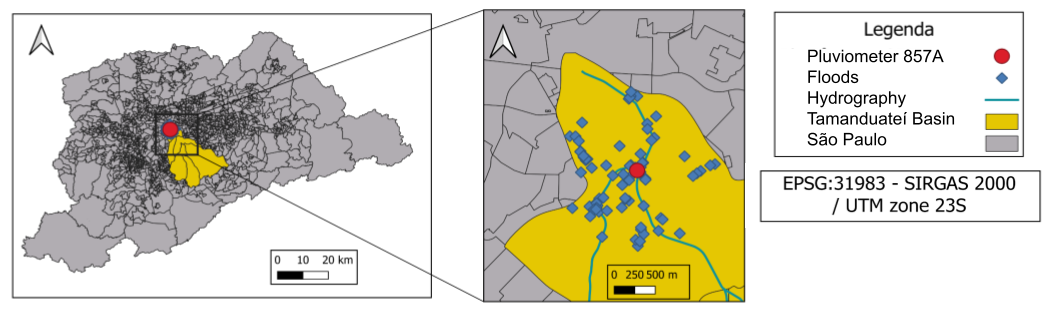
\includegraphics[scale=0.4]{imagens/ic_att2.png}
    \caption{�rea de estudo }
    \label{fig:area_estudo}
\end{figure}


Os dados da rede social Twitter foram extra�das atrav�s da API (\textit{Application Programming Interface}). Os dados pluviom�tricos s�o coletados do pluvi�metro 833A, pertencente ao Centro Nacional e Alertas e Desastres Naturais (CEMADEN), estes dados podem ser encontrados no pr�prio site da institui��o.  


A s�rie hist�rica de alagamentos na �rea de estudo, foram concebidas por um dos integrantes da pesquisa. Os dados metereol�gicos foram extra�dos por esta��es pertencentes ao CEMADEN, o equipamento est� localizado na cidade de S�o Roque - SP e atualmente est� em opera��o pelo Departamento de Controle do Espa�o A�reo (DECEA). Esse radar tem alcance de 250 km, cobrindo toda a regi�o metropolitana de S�o Paulo. O produto de radar usado para o CAPPI (Constant Altitude Plan Position Indicator) na altura de 3 km. Este produto possui uma resolu��o espacial de aproximadamente 1 km e uma resolu��o temporal de 10 minutos. Para a convers�o da refletividade (dBZ) em taxa de separa��o (mm / h) foi utilizado em rela��o a Marshall-Palmer \cite{marshall1948mc}) e a seguir os dados foram acumulados por dia. 

%%%%%%%%%%%%%%%%%%
\section{Ferramentas Computacionais}
A an�lise e aplica��o do projeto ser� realizada de maneira geral com a ferramenta \textit{Python}. Para a manipula��o, filtragem e tratamento dos dados ser� utilizada a biblioteca \textit{Pandas}, j� a an�lise gr�fica com \textit{Matplotlib} e \textit{Seaborn}. 


A aplica��o de testes estat�sticos na s�rie de dados ser� usado \textit{Scipy} e \textit{Numpy}, para os modelos de apredizagem supracitados, a biblioteca espec�fica para aprendizado de m�quina denominado \textit{Scikit-learn}. Por fim, algumas filtra��es no banco de dados de alagamentos ser� realizada com ferramentas de geoprocessamento do software \textit{QGIS}. 


%%%%%%%%%%%%%%%%%%
\section{Proposta de algoritmo para defini��o do modelo}
A concep��o inicial deste trabalho � analisar as s�ries temporais  dos alagamentos, tweets, pluvi�metro e radar, para definir quais s�o o melhor conjuntos de par�metros em dias de alagamentos, associando-se ao n�mero m�nimo necess�rio de tweets para emiss�o de um alerta. 


A s�rie temporal analisada compreende os tr�s primeiros meses do ano de 2019. Para a base de dados dos tweets, o processamento consiste no recorte temporal e filtra��o do tweets com base na lista de palavras associadas ao contexto metereol�gico e hidrol�gico. Esta lista de palavra basea-se no trabalho de \cite{de2021effect}. 


Com base na estrutura (Figura \ref{fig:metodologia}), ser� registrado em �nico arquivo, na mesma s�rie temporal, o n�mero de tweets filtrados, os valores de precipita��o do radar e o pluviom�tro, e se houve alagamentos no dias analisados. Este dados processados em um �nico arquivo, possibilitar�o a submiss�o nos modelos de aprendizados propostos, dividindo-se em base de dados para teste e treinamento.  
\begin{figure}[H]
    \centering
    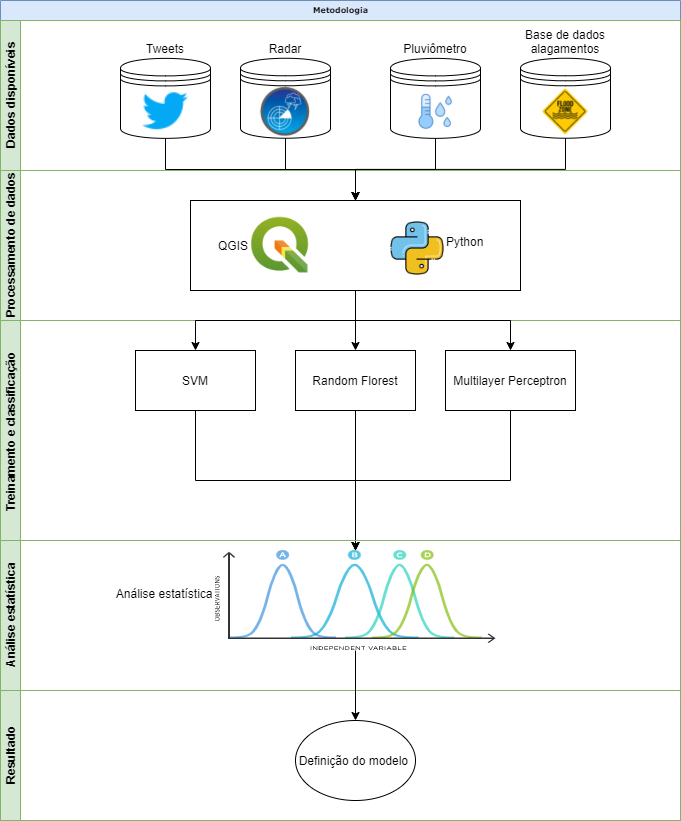
\includegraphics[scale=0.4]{imagens/medotologia.png}
    \caption{Metodologia}
    \label{fig:metodologia}
\end{figure}


Como a classifica��o bin�ria consiste em dias de alagamento e n�o alagamento, a acur�cia ser� medida a partir da base de dados de teste. Ap�s o treinamento nos modelo SVM e Floresta Aleat�ria e Redes Neurais, ser�o analisadas a acur�cia atrav�s da valida��o cruzada e subsequentemente testes estat�sticos como ANOVA e coeficiente Kappa, determinando-se assim, o algoritmo que possui maior potencial para o desenvolvimento de um sistema de alerta com base nos dados dispon�veis. 



%\section{Cronograma}
%A pesquisa ser� realizada em 12 meses e ser� executada nos passos listado abaixo (Tabela 1) \\ 
%A - Revis�o sistem�tica em desastres associados � alagamentos e modelos de classifica��o; \\
%B - Estudo dos modelos de aprendizado de m�quina e aplica��o em Python; \\
%C - Processamento dos bancos de dados; \\
%D - An�lise explorat�ria dos dados processados; \\
%E - Submiss�o dos dados processados para treinamento nos modelos propostos; \\
%F - Classifica��o; \\  
%G - C�lculos estat�sticos e infer�ncias;\\
%H - Altera��es, ajustes e otimiza��es no modelo de melhor desempenho; \\
%I - An�lise e conclus�o dos resultados; \\
%J - Relat�rio final 
%\begin{table}[H]
%    \centering
%    \begin{tabular}{|l|l|l|l|l|l|l|l|l|l|l|l|l|l|}
%\hline
%M�s &  & 1� & 2� & 3� & 4� & 5� & 6� & 7� & 8� & 9� & 10� & 11� & 12� \\ \hline
%\multirow{10}{*}{\begin{turn}{90} Etapas \end{turn}} & A & $\bullet$ & $\bullet$ &  &  &  &  &  &  &  &  &  &  \\ \cline{2-14} 
% & B & $\bullet$ & $\bullet$ & $\bullet$ &  &  &  &  &  &  &  &  &  \\ \cline{2-14} 
% & C &  &  & $\bullet$ & $\bullet$ &  &  &  &  &  &  &  &  \\ \cline{2-14} 
% & D &  &  &  & $\bullet$ &  &  &  &  &  &  &  &  \\ \cline{2-14} 
% & E &  &  &  &  & $\bullet$ & $\bullet$ &  &  &  &  &  &  \\ \cline{2-14} 
% & F &  &  &  &  & $\bullet$ & $\bullet$ &  &  &  &  &  &  \\ \cline{2-14} 
% & G &  &  &  &  &  &  & $\bullet$ & $\bullet$ &  &  &  &  \\ \cline{2-14} 
% & H &  &  &  &  &  &  &  & $\bullet$ & $\bullet$ &  &  &  \\ \cline{2-14} 
% & I &  &  &  &  &  &  &  &  &  & $\bullet$ & $\bullet$ &  \\ \cline{2-14} 
% & J &  &  &  &  &  &  &  &  &  &  & $\bullet$ & $\bullet$ \\ \hline
%\end{tabular}
%    \caption{Cronograma}
%    \label{tab:my_label}
%\end{table}



\newpage

\bibliographystyle{apalike}
\bibliography{bibliography.bib}

\end{document}